\chapter{Methods}
\label{ch:methods}

This chapter specifies the experiment. \secref{dg3-arch} describes the host model and the point where
the foveation attaches; \secref{eval-framework} fixes the dataset, the cross-validation partition and
the metrics; \secref{multi-subject} defines the per-image measures of human variability;
\secref{foveation} the input foveation itself; and \secref{training} the training protocol and the
analysis.

\section{The host and where the foveation attaches}
\label{sec:dg3-arch}

\chref{background} selected \dg{} as the host; \figref{dg3-published} is its architecture as the
authors drew it.

An image is first passed through a \textbf{DenseNet-201 backbone}, pretrained for object recognition on
sharp photographs and kept frozen. The read-out on top of it is built from a \textbf{saliency
network} of $1\times1$ convolutions (the \emph{spatial priority network} in \figref{dg3-published})
that turns the backbone features into a stimulus-driven map. A \textbf{scanpath network} encodes the last
four fixations, each as three maps holding, at every pixel, the distance to that fixation and its
horizontal and vertical components (\figref{dg3-published}b). A \textbf{fixation-selection network}
combines the two into one raw map.

The \textbf{Finalizer} turns that map into the output. It applies a learned Gaussian smoothing, adds a
log-centerbias prior, and normalises with a log-softmax, so the map exponentiates to a distribution over
the image. The result is the \emph{probability map} every later chapter reads, the probability at
each pixel that the next fixation lands there. The released \dg{} averages ten such read-outs, one per
cross-validation fold \citep{deepgazepytorch}; the foveation is shared by all ten.

The centerbias is a fixed map of where fixations land whatever the picture shows. Free-viewing gaze
concentrates near the centre of the stimulus \citep{tatler2007central}, and in MIT1003 $40\%$ of all
fixations fall in the central $11\%$ of the image area (\figref{judd-centerbias};
\citealp{judd2009mit1003}). Carrying it as a prior inside the Finalizer means the read-out does not have
to learn that tendency from the images.

\begin{figure}[tbp]
  \centering
  \begin{tikzpicture}
    \node[anchor=south west, inner sep=0] (dgimg)
      {
\includegraphics[width=0.99\textwidth]{kummerer2022_dg3_fig2.png}};
    \begin{scope}[x={(dgimg.south east)}, y={(dgimg.north west)}]
      \node[draw, very thick, rounded corners=2pt, fill=blue!15, align=center,
            font=\scriptsize\bfseries, inner sep=2.5pt] (fov) at (0.058,0.505)
        {foveation\\ \textnormal{\itshape (this thesis)}};
      \draw[-{Latex[length=2.2mm]}, very thick, blue!55!black] (fov.north) -- (0.058,0.625);
    \end{scope}
  \end{tikzpicture}
  \caption[\dg{}'s forward pass, with the foveation marked]{\dg{}'s forward pass. \textbf{(a)} The shaded box marks the input foveation of
    \secref{foveation}; everything after it is the published model. \textbf{(b)} The three maps each
    of the last four fixations becomes (two of the four drawn). \emph{Panels adapted from
    \citet{kummerer2022deepgaze3}, Figure~2.}}
  \label{fig:dg3-published}
\end{figure}

\begin{figure}[tbp]
  \centering
  
\includegraphics[width=0.44\textwidth]{judd2009_meanfixations.png}
  \caption[The MIT1003 centerbias]{All human fixations averaged over the 1003 MIT1003 images. The inner
    box covers the central $11\%$ of the image area and contains $40\%$ of all fixations, the outer box
    $25\%$ and $70\%$. Reproduced from \citet{judd2009mit1003}.}
  \label{fig:judd-centerbias}
\end{figure}

The foveation attaches before the backbone. The image is foveated, and everything downstream runs
unchanged. The comparison is clean because only the read-out carries trainable weights. Retraining under
a changed input (\secref{training}) adapts nothing else, so a measured difference is attributable to the
input rather than to a re-tuned backbone.

\section{Dataset and evaluation framework}
\label{sec:eval-framework}

Every quantitative result in this thesis comes from one evaluator, one dataset, and one fixed partition
of that dataset.

\subsection{The MIT1003 free-viewing dataset}
\label{subsec:mit1003}

The dataset used throughout is MIT1003 \citep{judd2009mit1003}. Its 1003 natural images were each freely
viewed for three seconds by up to fifteen subjects while eye position was recorded.

MIT1003 keeps each subject's scanpath separate and in viewing order, which the multi-subject analyses
of \secref{multi-subject} need.
It is also the dataset \dg{} was trained and benchmarked on \citep{kummerer2022deepgaze3}, so the
pretrained model is evaluated on the images it was fitted to.

The dataset is accessed through the \texttt{pysaliency} library (Appendix~\ref{app:data}).
Successive images were separated by one second of a gray screen, and every recorded scanpath begins with
a fixation at the image centre. \citet{judd2009mit1003} discard that initial centre fixation as trivial;
the variant loaded here keeps it, following the published \dg{} evaluation
\citep{kummerer2022deepgaze3}.
The centre fixation serves as history only, never as a target, and every free fixation is scored, which
gives $104{,}171$ fixations and puts the baseline on the protocol of the published figure.
Every arm is trained and scored under this protocol.

\subsection{Image-stratified cross-validation}
\label{subsec:cv-split}

The dataset is partitioned into ten folds of about $100$ images each. Every scanpath of an image
lands in the same fold, so a test image is never seen during training.
Each split takes eight folds for training, one for validation, and one for test
(Appendix~\ref{app:data}). The folds come from \texttt{pysaliency}'s cross-validation splitter, whose
fixed internal seed reproduces the partition the published \dg{} training notebook used
\citep{deepgazepytorch}.
Every arm of \secref{training} is trained ten times, once per fold, so an arm is ten models
(\figref{cv-split}).

\begin{figure}[tbp]
  \centering
  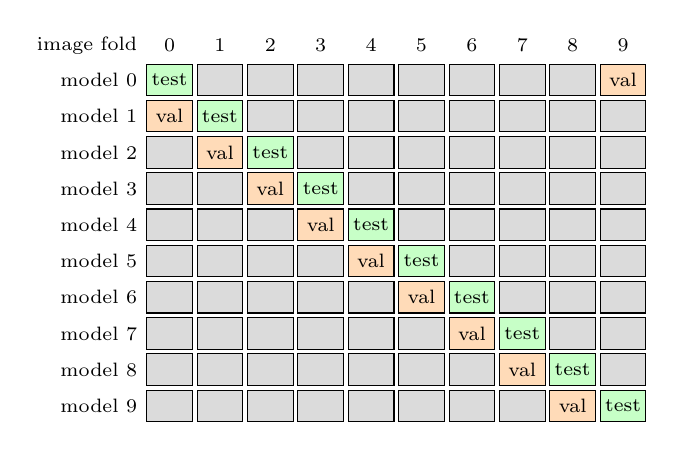
\begin{tikzpicture}[x=6.4mm, y=4.6mm, font=\scriptsize]
    \foreach \i in {0,...,9} { \node at (\i, 0.95) {\i}; }
    \node[anchor=east, font=\scriptsize] at (-0.45, 0.95) {image fold};
    \foreach \k in {0,...,9} {
      \node[anchor=east] at (-0.45, -\k) {model \k};
      \foreach \i in {0,...,9} {
        \pgfmathtruncatemacro{\isT}{ifthenelse(\i==\k,1,0)}
        \pgfmathtruncatemacro{\vv}{mod(\k+9,10)}
        \pgfmathtruncatemacro{\isV}{ifthenelse(\i==\vv,1,0)}
        \ifnum\isT=1
          \node[draw, fill=green!22, minimum width=5.8mm, minimum height=4.0mm, inner sep=0pt]
            at (\i,-\k) {test};
        \else
          \ifnum\isV=1
            \node[draw, fill=orange!28, minimum width=5.8mm, minimum height=4.0mm, inner sep=0pt]
              at (\i,-\k) {val};
          \else
            \node[draw, fill=black!14, minimum width=5.8mm, minimum height=4.0mm, inner sep=0pt]
              at (\i,-\k) {};
          \fi
        \fi
      }
    }
  \end{tikzpicture}
  \caption[The ten-fold image-stratified partition]{Each row is one of the ten models an arm consists of; every image is the test image of exactly
    one, so the ten test evaluations together cover the dataset once.}
  \label{fig:cv-split}
\end{figure}

The learning rate and the epoch the comparison is read at are chosen on the validation fold, and every
check that training behaved runs there. The test fold is scored after all training is complete, and it
is the source of the arm comparison in \chref{results}.

\subsection{Distribution-level performance metrics}
\label{subsec:metrics}

\dg{} outputs a probability map, the probability at each pixel that the next fixation lands there
(\secref{dg3-arch}).
All metrics are computed by reading this map at the pixel nearest each human fixation, never by comparing
scanpaths sampled from the model with human ones (\secref{models}; \citealp{kummerer2021state}).

Four metrics are computed per fixation, averaged per image and then over the images of a fold:
information gain, log-likelihood, NSS and AUC. Information gain is the primary one.
Throughout, an image has $H$ rows and $W$ columns, so $HW$ is its pixel count; $p(\vect{x})$ is the
probability the map puts on pixel $\vect{x}$; and $\vect{x}_1, \ldots, \vect{x}_n$ are the $n$ pixels
subjects were recorded fixating.

The \emph{log-likelihood} asks how much more probability the model put on those pixels than a map giving
every pixel the same value, $1/HW$. It is reported in \emph{bits per fixation}, where each bit doubles
the probability the model gave the pixel the subject chose, relative to a uniform map.

\begin{equation}
  \LL = \frac{1}{n} \sum_{i=1}^{n} \log_2 \frac{p(\vect{x}_i)}{1/HW}.
  \label{eq:ll}
\end{equation}

A uniform map is a weak reference, because free-viewing gaze concentrates near the image centre whatever
the picture shows. \emph{Information gain} is the same measurement with the reference swapped for the
centerbias, the prior that already knows about that tendency, so what remains is the information the
model adds beyond it \citep{kummerer2015information, kummerer2018benchmarking}:

\begin{equation}
  \IG = \LL_\text{model} - \LL_\text{centerbias},
  \label{eq:ig}
\end{equation}

also in bits per fixation, and zero for a model that adds nothing to the prior.
This is the measure \citet{kummerer2022deepgaze3} report for \dg{}.
The centerbias used here is the one distributed with the \dg{} release \citep{deepgazepytorch}, the same
prior the Finalizer adds (\secref{dg3-arch}), resized to each stimulus (Appendix~\ref{app:eval}).
\figref{scanpath-density} shows the maps \eqnref{ig} is read from along one scanpath, under the sharp
control and one foveated arm.

\begin{figure}[tbp]
  \centering
  \includegraphics[width=\textwidth, height=0.86\textheight, keepaspectratio]%
    {foveation_mit1003_initial/figs/scanpath_density_fov_cpd20_stim0091.png}
  \caption[One scanpath scored step by step]{The first five steps of one subject's scanpath on a held-out stimulus. The input column is the
    frame the foveated arm receives, re-centred on the current fixation (circle), with the subject's
    next saccade (arrow and star); each map is read at the pixel the subject moved to next, and
    averaging those terms over every scanpath in a fold is what the evaluator reports. The history is
    the subject's own fixations, never a path the model drew.}
  \label{fig:scanpath-density}
\end{figure}

NSS and AUC are not in bits and are reported alongside.
The normalised scanpath saliency \citep{peters2005nss},

\begin{equation}
  \NSS = \frac{1}{n} \sum_{i=1}^{n} \frac{p(\vect{x}_i) - \mu_p}{\sigma_p},
  \label{eq:nss}
\end{equation}

rescales the map to zero mean and unit standard deviation over its pixels ($\mu_p$ and $\sigma_p$) and
reads it where people looked, so it measures how much the model rated those places above its own
average.
The area-under-curve (AUC) metric asks a ranking question instead. Take a pixel someone fixated and a
pixel drawn at random from the same image; AUC is the probability the model rated the fixated one
higher:

\begin{equation}
  \AUC = \frac{1}{n\,HW} \sum_{i=1}^{n} \sum_{u=1}^{HW}
    \Big(\mathbf{1}\big[p(\vect{x}_i) > p_u\big]
       + \tfrac{1}{2}\,\mathbf{1}\big[p(\vect{x}_i) = p_u\big]\Big),
  \label{eq:auc}
\end{equation}

where the inner sum runs over every pixel $p_u$ of the image and $\mathbf{1}[\cdot]$ is the indicator
function, $1$ when the condition inside holds and $0$ otherwise. The discretised density makes exact
ties common, so they count half.
Only the order of the values matters, so AUC is unchanged by any rescaling of the map that preserves
it, and measures \emph{discrimination}, where the likelihood metrics reward getting the values
themselves right as well.
The shuffled-AUC variant is not used, because it draws its random pixels from other images' fixations
rather than uniformly, which divides the centerbias out \citep{kummerer2018benchmarking}, and that prior is
what \eqnref{ig} already measures against.

\section{Human variability and per-image difficulty}
\label{sec:multi-subject}
\label{subsec:difficulty-proxies}

Model fit varies widely between images, and the question here is what makes an image easy or hard. Human
agreement is the candidate, so the spread of the fifteen scanpaths has to be measured before it can be
correlated with anything.

The normalised Shannon entropy $H_{\text{fix}}$ of the population fixation density follows
\citet{judd2009mit1003}, who score per-image consistency as the entropy of the human fixation map pooled
over subjects; the version here bins the fixations rather than smoothing them.
All subjects' free fixations are pooled, binned into a $16 \times 16$ grid, and normalised to a probability
mass $p_k$ over the $K = 256$ cells,

\begin{equation}
  H_{\text{fix}} \;=\; -\frac{1}{\log_2 K} \sum_{k=1}^{K} p_k \log_2 p_k,
  \label{eq:fix-entropy}
\end{equation}

with $\log_2 K = 8$ putting $H_{\text{fix}}$ in $[0, 1]$. It rises as the population's gaze spreads.
\figref{entropy-panel} shows the quantity on the dataset's two extremes.

\begin{figure}[tbp]
  \centering
  
\includegraphics[width=\textwidth]{foveation_mit1003_initial/figs/entropy_panel.png}
  \caption[Fixation entropy at the dataset's extremes]{The stimulus where the subjects agreed most and the one where they agreed least, with their
    fixations, the same fixations counted into the $16 \times 16$ grid of \eqnref{fix-entropy}, and
    where both sit on the distribution over the 1003 stimuli.}
  \label{fig:entropy-panel}
\end{figure}

$H_{\text{fix}}$ is correlated against per-image model performance in \chref{results}. There the four
metrics of \subsecref{metrics} are computed per image, pooling only the subjects who viewed it. Both
Pearson's $r$ and Spearman's rank $\rho$ are reported.

\section{Gaze-contingent input foveation}
\label{sec:foveation}

\chref{background} introduced the acuity model; this section defines the transformation built on it:
the parametrised blur (\subsecref{gp-model}) and what its one strength parameter means against the
display and the dataset's saccades (\subsecref{sharp-radius}).
The fovea is re-centred on the most recent fixation of the history before every forward pass, in
training and in evaluation, so the foveation is \emph{gaze-contingent} and each pass sees the image as
a subject fixating there would.

\subsection{The blur and its parameters}
\label{subsec:gp-model}

The falloff is specified in degrees of visual angle, so its strength can be compared against measured
human acuity and carried unchanged across screen geometries.
Following \citet{geislerperry1998}, the highest spatial frequency resolvable at eccentricity $e$ (in
degrees) falls as

\begin{equation}
  f_c(e) \;=\; f_{c0}\,\frac{e_2}{e + e_2} \qquad [\text{cyc/deg}],
  \label{eq:gp-acuity}
\end{equation}

with foveal cutoff $f_{c0}$ and the half-acuity eccentricity fixed at $e_2 = 2.3^\circ$ in
\secref{foveated-vision}.
Their fitted contrast-threshold law puts the foveal cutoff at 39--41~cyc/deg
(Appendix~\ref{app:foveation}), so this work takes $f_{c0} = 40$~cyc/deg as the human setting.

$\ppd$ is how many pixels fit into one degree of visual angle on the subject's screen, set by screen
size, resolution, and viewing distance; for MIT1003, $\ppd = 35$ (Appendix~\ref{app:foveation}).
Dividing a pixel distance by $\ppd$ converts it to the degrees \eqnref{gp-acuity} expects,
$e_{\text{deg}} = e_{\text{px}} / \ppd$.

The naive way to apply the falloff is one blur per pixel. The image is foveated instead by blending a
Gaussian pyramid, a stack of uniformly-blurred copies built once per image, starting from the sharp
original and doubling the blur at each level. Every pixel is a linear interpolation between two levels,
so an image is blurred a few times instead of several hundred thousand.
The \emph{Nyquist} frequency is the highest frequency the display can carry, half its sampling rate,
here $0.5$~cyc/px.
For each pixel the target cutoff $f_c(e)$ of \eqnref{gp-acuity} is converted to cycles-per-pixel and
clamped at that limit; the corresponding fractional pyramid level is

\begin{equation}
  L(e) \;=\; \log_2\!\frac{0.5}{f_{c,\text{px}}(e)},
  \label{eq:frac-level}
\end{equation}

zero at the fovea and growing with eccentricity.
The foveated pixel is a linear interpolation between the two integer levels bracketing $L(e)$.
\figref{gp-pyramid} shows the construction; implementation detail is in Appendix~\ref{app:foveation}.

\begin{figure}[tbp]
  \centering
  
\includegraphics[width=\textwidth]{foveation_mit1003/figs/gp_pyramid.png}
  \caption[How the space-variant blur is built]{Top: the four shallowest pyramid levels on one patch, magnified because at full-frame size they
    are indistinguishable. Below, for each cutoff: the per-pixel level $L(e)$ of \eqnref{frac-level},
    dark where the frame stays sharp, and the foveated frame it produces.}
  \label{fig:gp-pyramid}
\end{figure}

The acuity profile forces one deviation from the published \dg{} protocol.
\citet{kummerer2022deepgaze3} resize every MIT1003 stimulus to $768 \times 1024$ or $1024 \times 768$.
Since the longest side is already $1024$~px, only the short axis stretches, and a stretched image turns
the sharp region around gaze into an ellipse rather than a disc.
This work therefore trains and evaluates at native resolution.
The released checkpoint was fitted on the resized stimuli, so native input is a mild distribution shift
for it.

\subsection{The sharp radius}
\label{subsec:sharp-radius}

At the MIT1003 geometry the Nyquist limit is $0.5\,\ppd = 17.5$~cyc/deg, and it is a property of the
display, so it is the same at every eccentricity.
Wherever $f_c(e)$ is above it the eye out-resolves the display, the clamp in \eqnref{frac-level} holds
$L$ at zero, and those pixels stay bit-identical to the sharp input; the fovea is therefore equally
sharp at every cutoff above the limit, and $f_{c0}$ controls how far out the sharp region reaches. At
$f_{c0} = 10$ the curve starts below the limit, so even the fovea is blurred.
Solving \eqnref{gp-acuity} for the eccentricity at which $f_c(e)$ meets the limit gives that radius in
closed form:

\begin{equation}
  e_{\text{sharp}} \;=\; e_2\!\left(\frac{2 f_{c0}}{\ppd} - 1\right) \quad [\text{degrees}]
  \quad\Longrightarrow\quad
  \ppd \cdot e_{\text{sharp}} \;=\; e_2\,(2 f_{c0} - \ppd) \quad [\text{pixels}].
  \label{eq:sharp-radius}
\end{equation}

At $f_{c0} = 40$ the sharp disc reaches $3.0^\circ$, while an MIT1003 stimulus spans
$29^\circ$ along its long side at $\ppd = 35$, so most of the frame is blurred at every cutoff.
Foveation strength is set by $f_{c0}$, with lower cutoffs blurring more.
\figref{foveation-strength} plots both sides of \eqnref{sharp-radius}, the crossing it solves and
the disc that crossing leaves on the frame.

\begin{figure}[tbp]
  \centering
  
\includegraphics[width=0.98\textwidth]{foveation_mit1003/figs/foveation_strength.png}
  \caption[The sharp radius]{The sharp radius at the three cutoffs of the arm list. Left: the falloff of \eqnref{gp-acuity}
    against the display Nyquist limit, with the crossing of \eqnref{sharp-radius} carried down to
    the axis; at $f_{c0} = 10$ the curve starts below the line, so that arm has no sharp disc. Right:
    the two remaining radii on stimulus~91, foveated at $f_{c0} = 40$ with the fovea at the image
    centre.}
  \label{fig:foveation-strength}
\end{figure}

The sharp disc reaches further than the fovea's $2^\circ$ (\secref{foveated-vision}) and than the
$e_2 = 2.3^\circ$ at which the eye's cutoff has halved, because the MIT1003 display carries only
$17.5$~cyc/deg and the eye does not fall to that until $3.0^\circ$. Out to that eccentricity a subject
out-resolves the screen, so blurring the image down to what the eye could see removes nothing that was
displayed. Given the acuity model, the sharp disc therefore follows from the display rather than from a
free parameter.

The sharp radius ties the strength sweep to the saccades the evaluator scores. Every scored
transition is a human saccade (\subsecref{metrics}), with a median amplitude of $155$~px ($4.4^\circ$
at $\ppd = 35$) over all $104{,}171$ of them, and \figref{saccade-coverage} reports for each cutoff the
fraction whose target falls inside the sharp disc and so reaches the backbone at full resolution:
$32.9\%$ at $f_{c0} = 40$, $0.6\%$ at $20$, and effectively none at $10$, where the disc has closed.

\begin{figure}[tbp]
  \centering
  
\includegraphics[width=0.94\textwidth]{foveation_mit1003/figs/saccade_coverage.png}
  \caption[Saccade amplitudes against the sharp radii]{The amplitudes of the $104{,}171$ saccades the
    evaluator scores, with the sharp radius of \eqnref{sharp-radius} marked for the two cutoffs that
    have one.}
  \label{fig:saccade-coverage}
\end{figure}

Between $40$ and $20$ the sharp disc shrinks past the typical saccade, so targets stop being delivered
sharp; between $20$ and $10$ almost no target is sharp in either arm, and any further cost comes
from how severely the target is blurred.
\figref{gp-strength} shows the strengths on four images, and the input column of
\figref{scanpath-density} the fovea moving down a subject's scanpath.

\begin{figure}[tbp]
  \centering
  
\includegraphics[width=\textwidth]{foveation_mit1003/figs/gp_strength_grid.png}
  \caption[Foveation strength on four stimuli]{Four MIT1003 images with the fovea held at the white dot, and the marked patch enlarged at each
    strength. Averaged over the four, the mean absolute change from the sharp original is $1.8/255$
    at $f_{c0} = 40$ and $5.6/255$ at $f_{c0} = 10$. The trained model re-centres the fovea on every
    fixation; it is held still here only to show strength.}
  \label{fig:gp-strength}
\end{figure}

\section{Training protocol: read-out fine-tuning on sharp versus foveated input}
\label{sec:training}

Networks fitted to sharp images lose accuracy under blur \citep{hendrycks2019robustness}, so \dg{} with
its pretrained read-out should be expected to underperform on foveated input. That penalty
measures the unfamiliarity of blurred input rather than what the removed detail was worth, so each arm
fine-tunes the read-out on its own input and the arms are compared after adaptation.
\subsecref{results-arms} reports what that penalty is before any fine-tuning.

\subsection{The arms}
\label{subsec:arms}

Every arm starts from pretrained \dg{} with the backbone and the Finalizer frozen (\secref{dg3-arch}),
and an audit asserts at construction that exactly the read-out is trainable (Appendix~\ref{app:training}).
The pretrained read-out is the released mixture of ten (\secref{dg3-arch}), each fitted on eight of these
same folds, and all ten are fine-tuned together, so a fold's test images were training data for most of
the read-outs its arms start from. Every arm shares that start, so the differences between arms are
unaffected; the absolute levels in \chref{results} are partly in-sample and sit above the published
cross-validated figure.

The cutoff $f_{c0}$ is swept from human acuity at $40$ down to $20$ and $10$~cyc/deg. One strength on
its own cannot separate a foveation that costs nothing from one too mild to measure, while a real cost
deepens as the periphery is degraded. Blur alone could produce such a cost, since the backbone was
pretrained on sharp photographs. Each cutoff therefore has a fixed-centre twin carrying the identical
blur pinned to the image centre, so the pair differs only in whether the sharp region follows the gaze.
With the sharp control, that makes the seven arms of \tabref{arms}.

Every arm is trained on all ten folds and shares the protocol (data, folds, optimiser, learning-rate
schedule, epoch count, seed, and the nearest-pixel target convention below), so the arms differ in
nothing but the input (Appendix~\ref{app:training}).

\begin{table}[tbp]
  \centering
  \caption[The seven arms]{The seven arms; only the input differs between them, and the sharp arm is the
    control every difference is taken against. The sharp radius sets what each cutoff is for
    (\subsecref{sharp-radius}): $f_{c0} = 40$ is human acuity and the main comparison, $20$ sits
    past the point where the sharp disc still covers a typical saccade, and $10$ is a coarse probe.}
  \label{tab:arms}
  \small
  \begin{tabular}{lcc}
    \toprule
    arm & fovea & $f_{c0}$ (cyc/deg) \\
    \midrule
    sharp (control)   & ---                          & --- \\
    \addlinespace[2pt]
    gaze-contingent   & follows the current fixation & $40$, $20$, $10$ \\
    \addlinespace[2pt]
    fixed-centre      & image centre                 & $40$, $20$, $10$ \\
    \bottomrule
  \end{tabular}
\end{table}

\subsection{Loss and optimisation}
\label{subsec:training-loop}

One training example is a \emph{(history, target) pair}, up to four fixations preceding some moment in one
subject's scanpath on one image and the location that subject moved to next.
The objective is the negative log-probability the model assigns to that location, identical to
\eqnref{ll} up to sign, base and a constant.
For a training image with $N_f$ such pairs, pooled across all subjects who viewed it,

\begin{equation}
  \mathcal{L}(\theta; \text{image})
  \;=\;
  -\frac{1}{N_f} \sum_{j=1}^{N_f} \log p_{\theta}(\vect{t}_j \mid \mathcal{H}_j, \text{image}),
  \label{eq:training-loss}
\end{equation}

with $\theta$ the trainable read-out parameters. The earliest pair of each scanpath predicts the first
free fixation from the centre fixation, as in the evaluator (\subsecref{mit1003}).
The target log-density is read at the pixel nearest $\vect{t}_j$, the same nearest-pixel lookup as in
evaluation (\subsecref{metrics}).

Optimisation is Adam over the read-out parameters, with the per-image loss accumulated in micro-batches
(Appendix~\ref{app:training}).
Each arm is trained for seven epochs at a base learning rate of $3 \times 10^{-4}$, divided by ten at
epoch five, the decaying schedule shape the \dg{} authors use.
The rate was chosen on validation and is shared by all seven arms, so
per-arm tuning cannot decide the comparison.

Epoch five is the highest in every arm, so it is the reporting epoch throughout and no per-arm choice
enters the comparison. It is also the first epoch after the decay, and epochs six and seven are run to
show that the curve flattens there rather than peaking, mean validation information gain changing by
less than $0.001$~bits per epoch across them in every arm (\figref{training-curves}).

Training runs on the Goethe-NHR cluster (Appendix~\ref{app:cluster}); the checkpoint format and gradient
clipping are in Appendix~\ref{app:training}.

\begin{figure}[tbp]
  \centering
  
\includegraphics[width=\textwidth]{foveation_mit1003_initial/figs/training_curves.png}
  \caption[Validation curves for the seven arms]{Top: validation information gain per epoch for the seven arms. The vertical line is the reporting
    epoch, the first trained at the decayed learning rate; the dashed line marks the decay and the
    labels give the rate each segment was trained at. Epoch $0$ is the pretrained read-out every arm starts from, scored by the evaluator of
    \secref{eval-framework} (the fixed-centre arms were not scored there). Bottom: the six foveated
    arms as fold-paired differences from the sharp control.}
  \label{fig:training-curves}
\end{figure}

\subsection{The comparison and its statistics}
\label{subsec:stats-plan}

The reported quantity is a difference in information gain between two arms at a given foveation strength,

\begin{equation}
  \Delta \IG \;=\; \IG_\text{arm} - \IG_\text{reference},
  \label{eq:delta-ig}
\end{equation}

with $\IG$ as in \eqnref{ig}.
The main comparison is the gaze-contingent arm at human acuity, $f_{c0} = 40$, against the sharp
control. The two coarser cutoffs test whether the cost grows as the falloff steepens, as
\secref{position} predicts if the periphery is what makes the next saccade choosable. The fixed-centre
arms hold the blur constant and take the gaze-contingency away. NSS, AUC and the diagnostics below are
reported alongside information gain.

Both arms see the same held-out fixations (\subsecref{cv-split}), so every difference is taken within an
image. Images vary much more in difficulty than the two arms differ from one another, and taking the
difference inside an image removes that variation.

Fixations from one image are not independent, coming from one scene and from the same people. Counting
each as its own observation would make the standard error too small. Each fold is averaged to a single
number first, which leaves ten.

The reported quantity is the mean of those ten differences. Every $\pm$ and every error bar in
\chref{results} is two standard errors of that mean.
Each arm and fold is one training run from seed $42$, so the interval carries fold-to-fold variation and
no run-to-run variation.

A likelihood reads the density at one pixel and says nothing about the rest of the map, so two arms can
score alike while failing in opposite ways, one spreading its mass and uncertain everywhere, the other
confident and pointing at the wrong place.
The \emph{entropy} of the predicted probability map, $-\sum p \log_2 p$ over all pixels, and the
\emph{mode distance} from the predicted peak to the true fixation separate them; the mode distance is
interpretable in pixels where bits are not.
Both are computed for both arms on identical scanpath positions, so the pairing is exact, and both are
reported as fold means, like the primary difference.
The difference of \eqnref{delta-ig} is also stratified, by saccade amplitude and by fixation index,
since a foveation effect should depend on how far the eye is moving and the earliest fixations are
centre-driven.
Two of the amplitude bin edges sit at the sharp radii of \eqnref{sharp-radius} ($11.5$~px at
$f_{c0} = 20$, $103.5$~px at $f_{c0} = 40$), so each bin lies wholly inside or wholly outside an arm's
sharp disc, and whether the cost appears where the disc ends can be read straight off the binned
differences.

These diagnostics are computed on the \emph{validation} split.
The test folds are reserved for the main comparison (\subsecref{cv-split}).


